\setcounter{section}{-1}
\section{Revision}

This course builds primarily on material on first- and second-order differential equations introduced in Several Variable Calculus and Differential Equations. In addition, some linear algebra - particularly the calculation of determinants, eigenvalues, and eigenvectors - is used as we study systems of ODEs expressed in matrix form.

\subsection{Matrices, Determinants, Eigenvalues, and Eigenvectors}

\begin{definition}
	The determinant of $A = \mat{a_{11} & a_{12} \\ a_{21} & a_{22}}$ is
	\[
	\det(A) = \abs{A} = \abs{\begin{array}{rr}a_{11} & a_{12} \\ a_{21} & a_{22}\end{array}} = a_{11}a_{22} - a_{12}a_{21}
	\]
\end{definition}

We then define the determinant of a $3 \times 3$ matrix in terms of determinants of $2 \times 2$ matrices.

\begin{definition}Let $A = \mat{a_{11} & a_{12} & a_{13} \\ a_{21} & a_{22} & a_{23} \\ a_{31} & a_{32} & a_{33}}$. Then the determinant of $A$ is the scalar
	\[
	\det(A) = \abs{A} = a_{11}\abs{\begin{array}{rr}a_{22} & a_{23} \\ a_{32} & a_{33}\end{array}} - a_{12}\abs{\begin{array}{rr}a_{21} & a_{23} \\ a_{31} & a_{33}\end{array}} + a_{13}\abs{\begin{array}{rr}a_{21} & a_{22} \\ a_{31} & a_{32}\end{array}}
	\]
\end{definition}

Given an $n \times n $ matrix $A$, the matrix $A_{ij}$ is nothing but $A$ with the $i$th row and $j$th column removed. The determinant of $A_{ij}$ is called a minor, and $C_{ij} = (-1)^{i+j} \det(A_{ij})$ is called a cofactor.

\begin{theorem}[The Laplace Expansion Theorem]
	The determinant of an $n \times n$ matrix $A = [a_{ij}]$, where $n \geq 2$, can be computed as
	\begin{align*}
		\det(A) &= a_{i1} C_{i1} + a_{i2} C_{i2} + \cdots + a_{in} C_{in} \\
		&= \sum_{j=1}^{n} a_{ij} C_{ij}.
	\end{align*}
	This is the cofactor expansion along the $i$th row. Alternatively,
	\begin{align*}
		\det(A) &= a_{1j} C_{1j} + a_{2j} C_{2j} + \cdots + a_{nj} C_{nj} \\
		&= \sum_{i=1}^{n} a_{ij} C_{ij}
	\end{align*}
	is the cofactor expansion along the $j$th column.
\end{theorem}

Since $C_{ij} = (-1)^{i+j} \det(A_{ij})$, each cofactor is plus or minus the corresponding minor, and the correct sign is given by the term $(-1)^{i+j}$. A quick way to remember which sign to use is to remember that the signs form a ``chequerboard'' pattern:
\[
\mat{+ & - & + & - & \cdots \\ - & + & - & + & \cdots \\ + & - & + & - & \cdots \\ - & + & - & + & \cdots \\ \vdots & \vdots & \vdots & \vdots & \ddots}
\]

Note that, if we are given the choice, then it will make sense to expand along the row or column with the most zero entries (i.e. fewest non-zero entries), as for each zero entry, we do not have to calculate the corresponding cofactor.

\begin{eg}Compute the determinant of
	\[
	A = \mat{2 & -3 & 0 & 1 \\ 5 & 4 & 2 & 0 \\ 1 & -1 & 0 & 3 \\ 2 & 1 & 0 & 0}
	\]
	Here, we note that we should expand along column 3 as it has only 1 non-zero entry.
	\begin{align*}
		\det(A) &= a_{13} C_{13} + a_{23} C_{23} + a_{33} C_{33} + a_{43} C_{43} \\
		&= 0(C_{13}) + a_{23} C_{23} + 0(C_{33}) + 0(C_{43}) \\
		&= -2 \abs{\begin{array}{rrr}2 & -3 & 1 \\ 1 & -1 & 3 \\ -2 & 1 & 0 \end{array}}
		\intertext{We now expand along the third row of the new determinant}
		&= -2 \left(-2 \abs{\begin{array}{rr}-3 & 1 \\ -1 & 3 \end{array}} - \abs{\begin{array}{rr}2 & 1 \\ 1 & 3 \end{array}} \right) \\
		&= -2(-2(-8) - 5) \\
		&= -22
	\end{align*}
\end{eg}

\begin{theorem}
	The determinant of a triangular matrix is the product of the entries on its main diagonal. Specifically, if $A = [a_{ij}]$ is an $n \times n$ triangular matrix, then
	\[
	\det(A) = a_{11} a_{22} \cdots a_{nn}
	\]
\end{theorem}

\begin{theorem}
	If $A$ and $B$ are $n \times n$ matrices, we have the following properties of determinants:
	\begin{align*}
		\det(kA) &= k^n \det(A) \\
		\det(AB) &= \det(A) \det(B) \\
		\det(A^{-1}) &= \frac{1}{\det(A)} \\
		\det(A) &= \det(A^T)
	\end{align*}
\end{theorem}

\begin{definition}
	Let $A$ be an $n \times n$ matrix. A scalar $\lambda$ is called an \vb{eigenvalue} of $A$ is there is a non-zero vector $\vbx$ such that $A\vbx = \lambda\vbx$. Such a vector $\vbx$ is called an \vb{eigenvector} of $A$ corresponding to $\lambda$.
\end{definition}

For a general $n \times n$ matrix $A$, the eigenvalues of this matrix are precisely the solutions $\lambda$ of the equation
\[
\det(A-\lambda I) = 0
\]

The procedure for finding eigenvalues and eigenvectors of a matrix is as follows:

Let $A$ be an $n \times n$ matrix:
\begin{enumerate}
	\item Compute the characteristic polynomial $\det(A - \lambda I)$ of $A$.
	\item Find the eigenvalues of $A$ by solving the characteristic equation $\det(A - \lambda I) = 0$ for $\lambda$.
	\item For each eigenvalues $\lambda$, find a corresponding eigenvector $\bm{v}$ by solving the system $(A-\lambda I)\bm{v} = \bm{0}$.
\end{enumerate}

\begin{eg}
	Find the eigenvalues and corresponding eigenspaces of
	\[
	A = \mat{0 & 1 & 0 \\ 0 & 0 & 1 \\ 2 & -5 & 4}
	\]
	
	First, the characteristic polynomial is
	\begin{align*}
		\det(A - \lambda I) &= \mat{-\lambda & 1 & 0 \\ 0 & -\lambda & 1 \\ 2 & -5 & 4-\lambda} \\
		&= \lambda \abs{\begin{array}{rr}-\lambda & 1 \\ -5 & 4-\lambda\end{array}} - \abs{\begin{array}{rr}0 & 1 \\ 4 & 4-\lambda\end{array}} \\
		&= \lambda(\lambda^2 - 4\lambda +5) - (-2) \\
		&= -\lambda^3 + 4\lambda^2 - 5\lambda + 2
	\end{align*}
	
	To find the eigenvalues, we solve $\det(A-\lambda I) =0$ for $\lambda$. The characteristic polynomial factors as $-(\lambda-1)^2(\lambda-2)$, so the solutions are $\lambda=1$ and $\lambda=2$. Since $\lambda=1$ is a repeated root and $\lambda=2$ is a simple root, we write $\lambda_1 = \lambda_2 = 1$ and $\lambda_3 = 2$.
	
	To find the eigenvectors corresponding to $\lambda_1 = \lambda_2 = 1$, we solve $(A-I)\bm{v} = \bm{0}$:
	\[
	\left(\begin{array}{r|r}A-I & 0\end{array}\right) = \left(\begin{array}{rrr|r}-1 & 1 & 0 & 0\\ 0 & -1 & 1 & 0 \\ 2 & -5 & 3 & 0\end{array}\right) \rightarrow \left(\begin{array}{rrr|r}1 & 0 & -1 & 0\\ 0 & 1 & -1 & 0 \\ 0 & 0 & 0 & 0\end{array}\right).
	\]
	By inspection, we an see that $\bm{v} = \mat{1\\1\\1}$ is an eigenvector.
	
	To find the eigenvectors corresponding to $\lambda_3 = 2$, we solve $(A-2I)\bm{v}=\bm{0}$:
	\[
	\left(\begin{array}{r|r}A-2I & 0\end{array}\right) = \left(\begin{array}{rrr|r}-2 & 1 & 0 & 0\\ 0 & -2 & 1 & 0 \\ 2 & -5 & 2 & 0\end{array}\right) \rightarrow \left(\begin{array}{rrr|r}1 & 0 & -\frac14 & 0\\ 0 & 1 & -\frac12 & 0 \\ 0 & 0 & 0 & 0\end{array}\right),
	\]
	from which we can see that $\bm{v} = \mat{1\\2\\4}$ is an eigenvector.
\end{eg}

We define \vb{algebraic multiplicity} of an eigenvalue to be its multiplicity as a root of the characteristic equation. Thus, in the previous example, $\lambda=1$ would have algebraic multiplicity 2 and $\lambda=2$ algebraic multiplicity 1.

We then define the \vb{geometric multiplicity} of an eigenvalue $\lambda$ to be the number of linearly independent eigenvectors. So $\lambda=1$ and $\lambda=2$ both have geometric multiplicity 1.


\subsection{First-Order ODEs}

A separable first-order ODE of the form
\begin{equation}
	\frac{dy}{dx} = \frac{f(x)}{g(y)}, \quad y(0) = y_0,
\end{equation}
can be solved by integration:
\[
\int g(y) \,dy = \int f(x) \,dx.
\]

Linear first-order ODEs of the form
\begin{equation}
	y' + p(x)y = g(x)
\end{equation}
can be solved using the method of integrating factors. With this method, we multiply the original ODE by the integrating factor
\[
I(x) = \exp \int p(x)\,dx.
\]
The resulting ODE can be written as
\begin{align*}
	I(x)y' + p(x)I(x)y &= I(x)g(x) \\
	\frac{d}{dx}(I(x)y) &= I(x)g(x)
\end{align*}
Integrating both sides with respect to $x$ yields
\[
y = \frac{1}{I(x)}\left[\int I(x)g(x) \,dx + C\right].
\]

\subsection{Second-Order Linear ODEs}\label{sec:secondorderconst}

The solution of homogeneous second-order linear constant-coefficient ODEs
\begin{equation}\label{eq:revisionhom}
	ay'' + by' + cy = 0
\end{equation}
can be sought by trying exponential solutions $y = e^{rx}$. This leads to the characteristic equation
\[
ar^2 + br + c = 0
\]
for $r$. We find the roots of this trinomial to be $r_1$ and $r_2$, then the general solution is found from one of the following three cases:
\begin{itemize}
	\item In the case of $r_1$ and $r_2$ being real and distinct, the general solution is
	\[
	y(x) = C_1e^{r_1x} + C_2e^{r_2x}.
	\]
	\item In the case that there is a repeated root $r=r_1=r_2$, the general solution is
	\[
	y(x) = (C_1 + C_2x)e^{rx}.
	\]
	\item If the characteristic equation has complex roots, the roots come in a complex-conjugate pair, $r = \lambda \pm i\mu$ and the general solution is
	\[
	y(x) = e^{\lambda x}(C_1 \cos(\mu t) + C_2 \sin(\mu t)).
	\]
\end{itemize}

The solution of a non-homogeneous second-order constant-coefficient ODE
\begin{equation}\label{eq:revisionnonhom}
	ay'' + by' + cy = g(x)
\end{equation}
is found as the superposition of the solution to the homogeneous equation and a particular solution, $y_p(x)$ of the inhomogeneous equation, e.g.
\[
y(x) = C_1e^{r_1x} + C_2e^{r_2x} + y_p(x)
\]

The particular solution can be found by
\begin{itemize}
	\item Method of undetermined coefficients when $g(x)$ is a polynomial, exponential, sine or cosine, or a product of these.
	
	With this method, we make an educated guess as to the particular solution, e.g. $y_p(x) = Ae^{2x}$ if $g(x) = 5e^{2x}$, then find the derivatives $y_p'$ and $y_p''$. We can substitute these into \Cref{eq:revisionnonhom} to solve for the undetermined coefficients ($A$ in this example). The following are general rules for picking the trial function:
	\begin{enumerate}[label=(\roman*)]
		\item If $g(t) = Me^{kt}$,
		\begin{itemize}
			\item Try $y_p(t) = Ce^{kt}$ if $k$ is not a root of the characteristic equation.
			\item Try $y_p(t) = Cte^{kt}$ if $k$ is a root of the characteristic equation.
			\item Try $y_p(t) = Ct^2e^{kt}$ if $k$ is a repeated root of the characteristic equation.
		\end{itemize}
		\item If $g(t) = M\cos(kt) + N\sin(kt)$ (including if $M$ or $N$ is zero),
		\begin{itemize}
			\item Try $y_p(t) = C\cos(kt) + D\sin(kt)$ if $\pm ik$ are not roots of the characteristic equation.
			\item Try $y_p(t) = t(C\cos(kt) + D\sin(kt))$ if $\pm ik$ are roots of the characteristic equation.
		\end{itemize}
		\item If $g(t) = a_nt^n + a_{n-1}t^{n-1} + \cdots + a_1t + a_0$,
		\begin{itemize}
			\item Try $y_p(t) = b_nt^n + \cdots + b_1t + b_0$ if 0 is not a root of the characteristic equation.
			\item Try $y_p(t) = t(b_nt^n + \cdots + b_1t + b_0)$ if 0 is a root of the characteristic equation.
			\item Try $y_p(t) = t^2(b_nt^n + \cdots + b_1t + b_0)$ if 0 is a repeated root of the characteristic equation.
		\end{itemize}
		\item In the case where $g(t)$ is a product of a polynomial, exponential, and/or trigonometric function, the trial function is nothing but the product of the relevant trial functions from cases (i) to (iii). For example, if $g(t) = e^{2t}\sin(3t)$, we would try $y_p(t) = e^{2t}(A\sin(3t) + B\cos(3t))$. The only caveat is that we may need to multiply by $t$ or $t^2$ to ensure that no term in the trial function appears in the homogeneous solution.
	\end{enumerate}
	
	\item Variation of parameters, for any $g(x)$. If $y_1(x)$ and $y_2(x)$ are solutions to the homogeneous ODE in \Cref{eq:revisionhom}, then the particular solution of \Cref{eq:revisionnonhom} is
	\[
	y_p(x) = -y_1(x)\int\frac{y_2(x)g(x)}{aW(y_1,y_2)}\,dx + y_2(x)\int\frac{y_1(x)g(x)}{aW(y_1,y_2)}\,dx.
	\]
	where the Wronskian $W(y_1,y_2)$ is given by
	\[
	W(y_1, y_2) = \det\mat{y_1 & y_2 \\ y_1' & y_2'}.
	\]
\end{itemize}

\begin{figure}
	\centering
	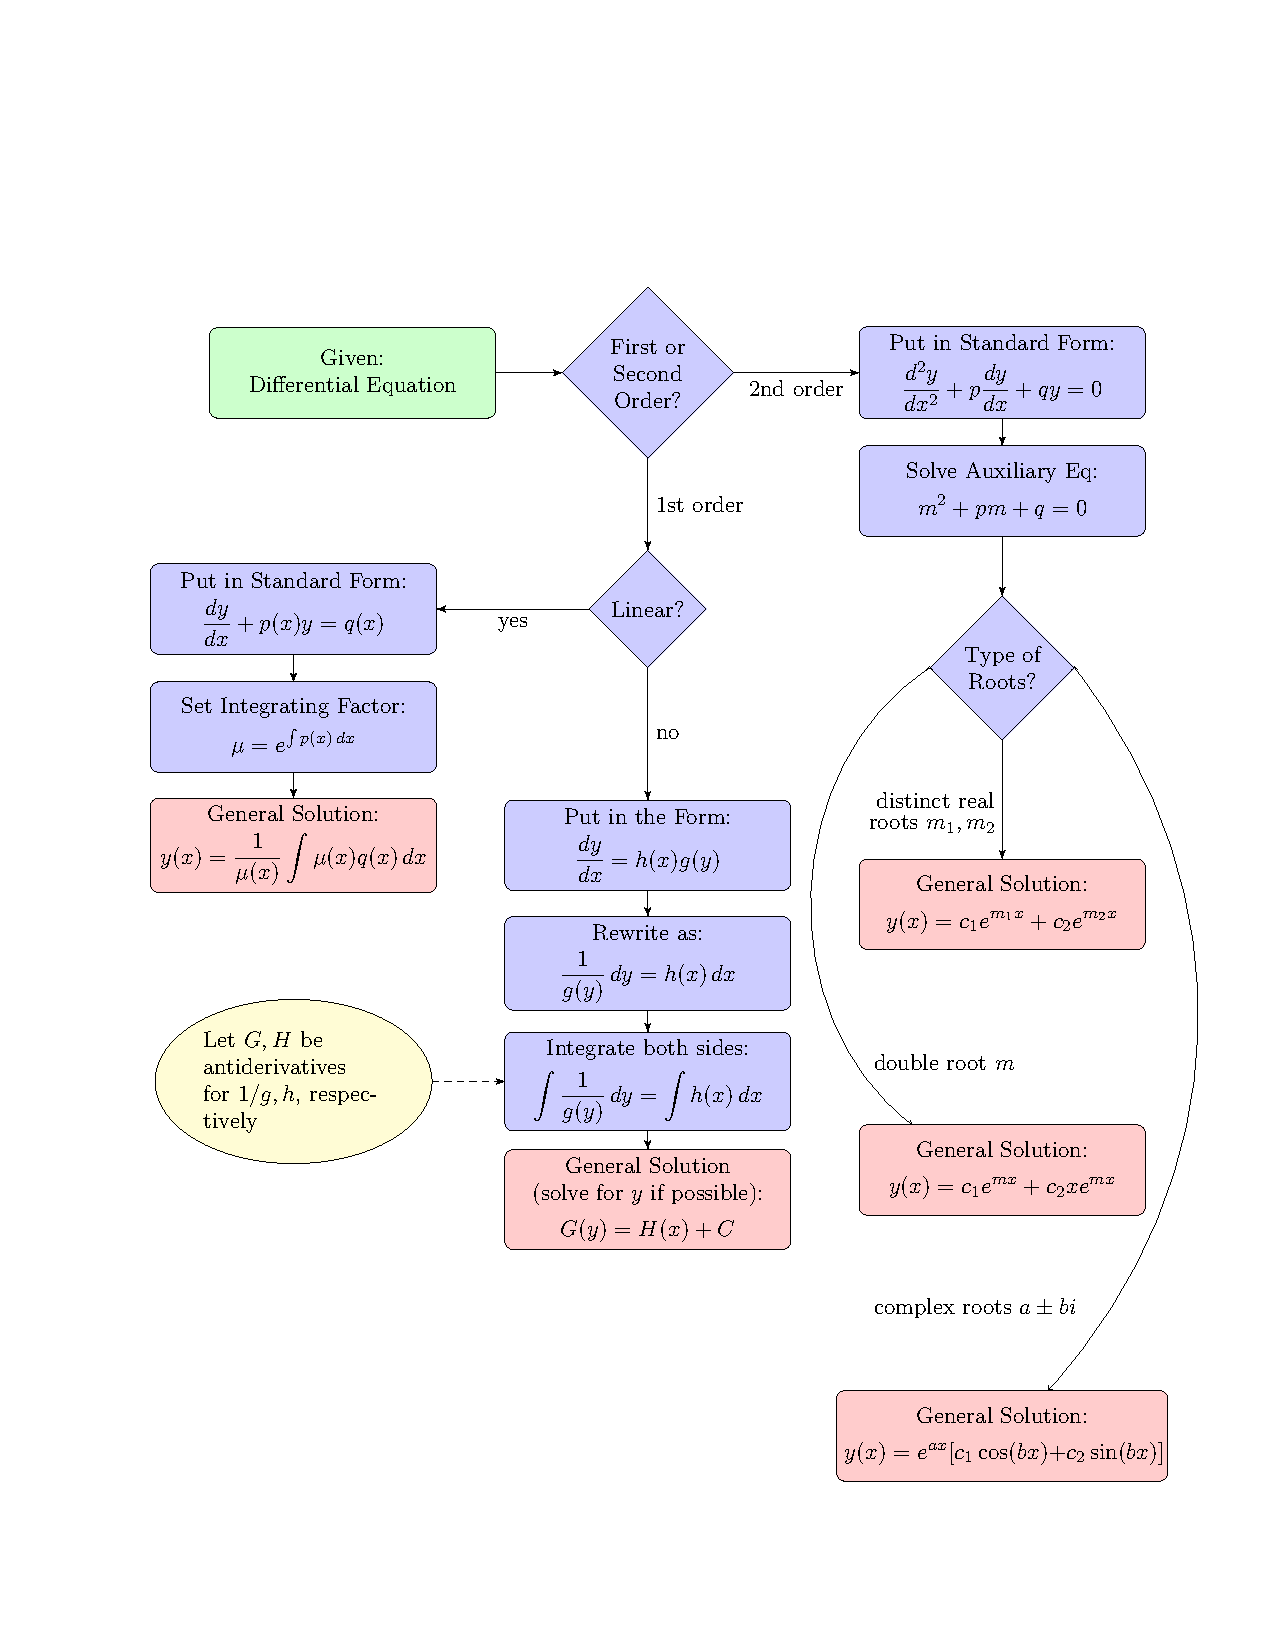
\includegraphics[width=\linewidth]{img/RevisionFlowchart}
	\caption{Flowchart for solving first and second order ODEs. \href{http://courses.enriqueareyan.com/files/math/M343\%20Introduction\%20to\%20Differential\%20Equations\%20I/Resources/DifferentialEquations-Flowchart.pdf}{Source}.}
	\label{fig:revisionflowchart}
\end{figure}

% https://matheducators.stackexchange.com/questions/16825/diagram-of-methods-to-solve-differential-equations